\section{Controlled Experiments}
\label{sec:controlled_experiments}

\subsection{Implementation identity and experimental design}
We use E1 to examine bandwidth sharing between two flows of the same
implementation as RTT asymmetry and queue depth change, and E2 to examine
coexistence with CUBIC. E3 extends the equal-RTT comparison across capacity
and propagation delay. An artificial-loss extension separates configured
access-link loss from bottleneck congestion. These tests evaluate the
framework's assessment dimensions under stated conditions, Each experiment addresses a separate assessment question.

The Linux emulation uses Mininet 2.3.0, Open vSwitch bridges, iperf3 3.9
and iproute2 5.15.0. Two sender hosts connect through switches $s_1$ and
$s_2$ to one receiver: $h_1,h_2\rightarrow s_1\rightarrow s_2\rightarrow h_3$.
The $s_1$--$s_2$ link is the bottleneck, configured with a token-bucket
rate limiter and child netem FIFO packet limit, without AQM or ECN.
The receiver access link supplies the base propagation delay; additional
delay on the second sender's access link creates RTT asymmetry. Each
sender opens one TCP connection to a separate receiver port (5201 or
5202), with one-second iperf3 reporting intervals. The topology is rebuilt
between runs. The MTU is 1,500 bytes. In E1/E2, the reference BDP is
$100\,\mathrm{Mbps}\times20\,\mathrm{ms}/8=250,000$ bytes, using the first
flow's configured propagation RTT, including when the second RTT differs.
Queue targets of 125,000, 500,000 and 2,500,000 bytes are rounded up to
84, 334 and 1,667 MTU-sized packets, respectively.

The archived experiments comprise 340 two-flow runs: 60 each for the
Ubuntu 5.15.0-181-generic in-tree baseline, the separately loaded BBRv1 module, BBR2, and
BBRv3; 80 E3 runs; and 20 artificial-loss runs. The manifests identify
BBRv3 by the 6.13.7-bbr3 kernel, source marker BBR\_VERSION=3, and runtime
name \texttt{bbr}. The BBRv1 module registers as \texttt{bbr1} and uses
a recorded compatibility patch for an unexported TSO helper. BBR2 uses
a separate 5.13.12-bbr2alpha kernel and runtime name \texttt{bbr2}.
The in-tree baseline remains a distinct implementation label.
Different kernel environments and the module patch limit causal
attribution of performance differences to algorithm version alone.

The E1/E2 matrix uses a 100-Mbps bottleneck, a 20-ms first-flow RTT,
second-flow RTTs of 20, 40, or 80 ms for the same-algorithm comparison,
and equal-RTT BBR/CUBIC competition. Queue targets are 0.5, 2, or 10
times the reference BDP. Each condition has five 180-s repetitions,
with ECN disabled. Receiver-side iperf3 summaries provide the archived
full-run goodput. Jain fairness and flow shares are derived from those
per-flow rates. For each run, with receiver rates $x_1,x_2$, we compute
$G=x_1+x_2$, $J=(x_1+x_2)^2/[2(x_1^2+x_2^2)]$ and
$S_2=x_2/(x_1+x_2)$. Reported Jain indices and shares are means of
these run-level quantities, rather than values calculated from mean rates.
In E2, flow 1 is BBR and flow 2 is CUBIC, so the mean BBR share is
$1-\overline{S_2}$. Receiver goodput excludes protocol headers; therefore
it need not equal the configured link rate. The supplement supplies
per-run values and variability; five repetitions support descriptive
comparisons, not population-wide significance claims.

The configuration declares a 30-s warmup; the primary archived analysis
uses the complete receiver summary. A separate sensitivity analysis uses
complete receiver intervals within the configured 30--180-s window,
without estimating bytes in boundary intervals. Across 68 condition
summaries, the largest absolute changes in mean total goodput, Jain
index, and second-flow share are 1.313 Mbps, 0.02949, and 0.01678,
respectively. The separate window analysis quantifies the sensitivity of these summaries.

Loaded RTT measurements are sequential early ping samples from the two
senders. Queue counters were sampled before the transfers completed.
The RTT and queue observations use different windows from the receiver
goodput summary; their values are reported as complementary measurements.

\subsection{Conditioned cross-version comparison}
Across the tested 100-Mbps matrix, equal-RTT total goodput remains close to
the bottleneck for all four implementations, while flow shares and Jain
fairness vary with RTT asymmetry, queue setting, and implementation. Under
the 40- and 80-ms second-flow conditions, the observed long-RTT share differs across implementations. E1 quantifies allocation under RTT asymmetry; E2 evaluates coexistence
with CUBIC at equal RTTs in the documented implementation environments.

For the no-ECN BBR/CUBIC comparison, total goodput is similar across the
four implementation environments, while the BBR/CUBIC share and Jain
index remain condition dependent. The experimental supplement contains the per-run rates, condition
summaries and plotting scripts.

\begin{figure}[htbp]
\centering
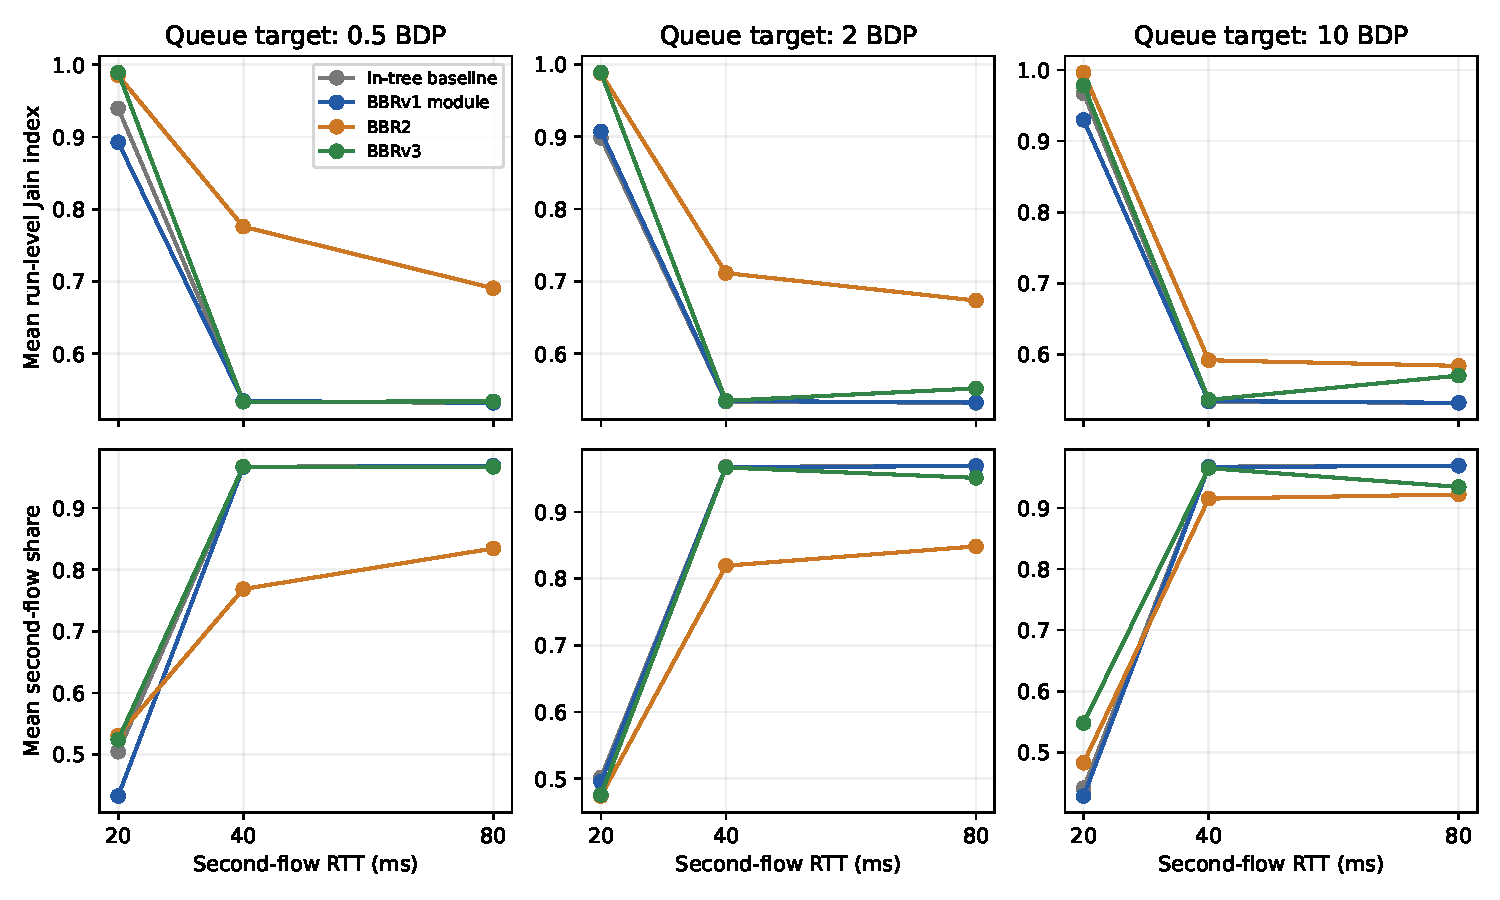
\includegraphics[width=\linewidth]{e1_results.pdf}
\caption{E1 two-flow comparison at 100 Mbps, with first-flow RTT 20 ms and ECN disabled. Curves show means of five run-level Jain indices and second-flow shares, not indices computed from averaged rates. Queue targets use the reference BDP.}
\label{fig:e1_results}
\end{figure}

\begin{table}[htbp]
\centering
\caption{E2 competition with CUBIC at 100 Mbps and equal 20-ms RTTs, with ECN disabled. Each cell summarizes five full-run receiver measurements. Share denotes the BBR flow; Jain is the mean of per-run indices. Different implementation environments limit causal version attribution.}
\label{tab:e2_results}
\small
\begin{tabular}{lrrrr}
\toprule
Implementation & Q/BDP & Total (Mbps) & BBR share & Jain \\
\midrule
In-tree baseline & 0.5 & 95.59 & 0.155 & 0.677 \\
In-tree baseline & 2 & 95.59 & 0.153 & 0.674 \\
In-tree baseline & 10 & 95.58 & 0.165 & 0.690 \\
BBRv1 module & 0.5 & 95.59 & 0.144 & 0.663 \\
BBRv1 module & 2 & 95.59 & 0.143 & 0.663 \\
BBRv1 module & 10 & 95.59 & 0.149 & 0.669 \\
BBR2 & 0.5 & 95.58 & 0.278 & 0.835 \\
BBR2 & 2 & 95.58 & 0.327 & 0.886 \\
BBR2 & 10 & 95.58 & 0.274 & 0.828 \\
BBRv3 & 0.5 & 95.58 & 0.153 & 0.675 \\
BBRv3 & 2 & 95.58 & 0.145 & 0.664 \\
BBRv3 & 10 & 95.59 & 0.164 & 0.689 \\
\bottomrule
\end{tabular}
\end{table}


Table~\ref{tab:e2_results} shows that similar total goodput does not imply
similar bandwidth allocation. Total rates are 95.58--95.59 Mbps in this
matrix, while the BBR share is 0.143--0.327. BBR2 obtains shares of
0.274--0.327 and Jain indices of 0.828--0.886; the BBRv1 module and
BBRv3 obtain smaller shares in these particular runs. The implementation environments and no-ECN configuration identify the
scope of these comparisons.

For unequal-RTT E1 cases, the second flow receives substantially more than
half the goodput in the tested matrix (Figure~\ref{fig:e1_results}). The
size of the imbalance varies with implementation and queue setting: across
the 24 unequal-RTT conditions, the mean long-RTT share ranges from
0.769 to 0.969, and mean Jain fairness from 0.532 to 0.776.
These measured shares make allocation an explicit assessment outcome,
alongside the aggregate rate and the reported path conditions.

\subsection{Additional comparison under equal RTT}
The additional experiment matrix contains eight network cases at 50 or
200~Mbps, 10 or 60~ms RTT, and two frozen buffer labels.
For the 50-Mbps cases, the configured absolute buffers correspond
to 4 and 16 times the physical reference BDP, although the frozen file
labels them 1 and 4. For the 200-Mbps cases, those labels are consistent
with the capacity-times-reference-RTT BDP. The original predictions
are retained; the affected cases do not validate the intended buffer bins. We ran two BBRv3 flows
and two CUBIC flows separately for five independent repetitions per case
(80 runs in total). ECN is disabled in all cases.

Table~\ref{tab:e3_candidate} reports mean total goodput and Jain fairness.
E3 extends the rate/fairness assessment across two capacities and two
RTTs. Mean BBRv3 Jain indices range from 0.995 to 1.000, compared with
0.917 to 0.987 for CUBIC; the table reports the corresponding goodput
values together, making both utilization and sharing visible. The queue snapshots do not cover the complete measurement window;
The receiver summary, sender retransmissions and queue snapshot provide
separate indicators for the documented operating conditions.
The archived goodput and Jain values use full-run receiver summaries.
A separate post-warmup interval sensitivity analysis is retained;
the table reports the complete receiver summary; window sensitivity is
provided separately.

\begin{table}[htbp]
\centering
\caption{Descriptive E3 full-run means. Goodput (Mbps) and Jain cells report BBRv3/CUBIC. C is Mbps and RTT is ms. Buffer uses decimal kB; actual target Q/BDP is computed from capacity and reference RTT, before packet-limit rounding. Frozen labels are preserved in the input audit.}
\label{tab:e3_candidate}
\begin{tabular}{lrrrrrr}
\toprule
Case & C & RTT & Buffer (kB) & Actual Q/BDP & Goodput & Jain \\
\midrule
E3\_001 & 50 & 10 & 250 & 4 & 47.1/47.8 & 1.000/0.969 \\
E3\_002 & 50 & 10 & 1000 & 16 & 47.2/47.8 & 1.000/0.917 \\
E3\_003 & 50 & 60 & 1500 & 4 & 46.9/47.7 & 1.000/0.928 \\
E3\_004 & 50 & 60 & 6000 & 16 & 46.8/47.7 & 1.000/0.987 \\
E3\_005 & 200 & 10 & 250 & 1 & 188.2/191.2 & 0.995/0.963 \\
E3\_006 & 200 & 10 & 1000 & 4 & 188.0/191.2 & 0.999/0.955 \\
E3\_007 & 200 & 60 & 1500 & 1 & 187.0/190.8 & 0.997/0.963 \\
E3\_008 & 200 & 60 & 6000 & 4 & 187.1/190.8 & 0.996/0.938 \\
\bottomrule
\end{tabular}
\end{table}


\subsection{Goodput under artificial access-link loss}
The artificial-loss extension compares BBRv3 and CUBIC at configured
loss probabilities of zero and 0.1\% on a separate access link. Each run
uses two flows of the same algorithm, a 100-Mbps bottleneck, equal 20-ms
RTTs and a 500,000-byte queue target (2 reference BDP),
with five runs per algorithm and loss setting. Archived full-run mean total
goodput changes from 93.87 to 94.25 Mbps for BBRv3 and from 95.58 to
81.06 Mbps for CUBIC. The small BBRv3 increase is a descriptive observation
and is not evidence that loss improves performance. The loss generator's
seed was not exposed in the retained configuration; this setup does not
represent correlated wireless or satellite errors.

The additional equal-RTT cases extend the capacity and RTT settings of
the main matrix. Their physical queue sizes are reported explicitly in
Table~\ref{tab:e3_candidate}. Because four cases differ from the intended
buffer labels, we use these results as an additional empirical comparison,
rather than as a validation of the original buffer-category predictions.
The experiments evaluate goodput and bandwidth sharing under controlled
conditions; they do not establish universal suitability thresholds or
isolate the causal effect of an individual controller mechanism.

\subsection{Quantitative Transfer Evaluation of the Framework}
\label{sec:framework_transfer}

We supplement the scenario comparisons with a quantitative test of whether
an equal-RTT calibration transfers to different capacities and delays.
This analysis was designed during revision after the archived results were
available. Calibration and evaluation runs are disjoint, but the test is
retrospective; its design and data split are documented in the supplement.
The analysis script retains all inputs and reports the constant-baseline
comparison, including the contribution of queue conditioning.

Calibration uses only the 15 BBRv3 E1 runs with equal 20-ms RTTs at
100 Mbps, five at each queue target $q\in\{0.5,2,10\}$. At each target,
we estimate mean $u$ and mean $J$. For a target queue ratio between knots,
we linearly interpolate the two means in $\log q$; outside the range,
we extend the adjacent segment and restrict predictions to the metric's
feasible interval. The comparator predicts the overall calibration mean,
independent of queue size. Neither model fits an E3 outcome. Capacity and
RTT effects cannot be estimated from this single-capacity, equal-RTT
calibration; transferring normalized rates therefore tests an explicit
assumption that the evaluation tests.

The primary transfer comparison uses the four 200-Mbps E3 cases, where
physical queue ratios agree with the frozen input labels: RTTs of 10 or
60 ms and $q\in\{1,4\}$. The four 50-Mbps cases are a separate comparison
using their corrected physical ratios of 4 and 16. Errors are computed
against each condition's five-run mean, for 20 BBRv3 runs in each group.
The 40 CUBIC runs remain a performance comparator and are not calibration
data for the BBRv3 predictor.

\begin{table}[htbp]
\centering
\small
\caption{Retrospective transfer errors for BBRv3 condition means. MAE is the
mean absolute error; normalized-goodput errors are fractions of capacity.
Queue interpolation uses E1 only. The constant predictor uses the same
calibration data. Each row evaluates four E3 conditions.}
\label{tab:framework_transfer}
\begin{tabular}{llrrr}
\toprule
Evaluation group & Metric & Queue MAE & Constant MAE & Queue max. error \\
\midrule
200 Mbps, actual $q=1,4$ & $u$ & 0.00264 & 0.00264 & 0.00400 \\
 & $J$ & 0.01010 & 0.01134 & 0.01464 \\
50 Mbps, actual $q=4,16$ & $u$ & 0.00309 & 0.00309 & 0.00366 \\
 & $J$ & 0.02027 & 0.01444 & 0.02499 \\
\bottomrule
\end{tabular}
\end{table}

Table~\ref{tab:framework_transfer} separates modest transfer error from
predictive added value. In the four input-matched cases, the queue-conditioned
Jain estimate has slightly smaller MAE than the constant predictor, but
normalized-goodput MAE is the same to the displayed precision. In the corrected 50-Mbps cases, Jain MAE is 0.02027 for queue
interpolation and 0.01444 for the constant estimate. This comparison
identifies the dependence of transfer estimates on their conditioning
variables. The largest Jain error is about
0.025; reporting only high aggregate utilization would conceal this
assessment limitation. These results quantify the framework's transfer
boundary without claiming that E3 validates the original queue thresholds.

We also instantiate the analytical assessment in
Section~\ref{sec:analytical_assessment} with illustrative requirements
$u_0=0.90$ and $j_0=0.95$. These values were selected for retrospective
illustration, not frozen as experimental acceptance thresholds. All 40
BBRv3 and all 40 CUBIC E3 runs meet the utilization requirement, while
40 BBRv3 and 27 CUBIC runs meet both requirements. The result is restricted
to equal-RTT same-algorithm competition; E2 provides the separate coexistence
assessment. The supplement reports
run-level decisions and a threshold sensitivity grid. Receiver-goodput and early-ping windows are reported separately. Sender
retransmission totals and queue snapshots provide complementary indicators
for the documented operating conditions.

\begin{table}[htbp]
\centering
\small
\caption{Sensitivity of the retrospective E3 rate/fairness assessment to
illustrative service requirements. Cells count runs meeting both limits,
from 40 runs per algorithm. They are not independent condition counts.}
\label{tab:assessment_requirements}
\begin{tabular}{rrrr}
\toprule
Minimum $u$ & Minimum $J$ & BBRv3 & CUBIC \\
\midrule
0.90 & 0.95 & 40/40 & 27/40 \\
0.95 & 0.95 & 0/40 & 27/40 \\
0.90 & 0.99 & 38/40 & 19/40 \\
\bottomrule
\end{tabular}
\end{table}

The higher utilization requirement in Table~\ref{tab:assessment_requirements}
reverses which algorithm meets the joint requirement more often: no
BBRv3 run reaches $u=0.95$, whereas all CUBIC runs do. Tightening fairness
instead reduces both algorithms' pass counts. This measured throughput--allocation tradeoff makes the service
preference explicit under equal RTTs. The full
threshold grid and per-condition variability are provided in the supplement.

The frozen F07 predictions are retained separately from this new analysis.
They specify qualitative ``near-capacity'' or ``near-one'' outcomes without
numerical acceptance margins, and request medians rather than the reported
full-run means. Four cases also have inconsistent physical queue inputs.
The new transfer test reports numerical error directly; the historical
prediction sheet remains in the supplement as a separate record.

